% Options for packages loaded elsewhere
\PassOptionsToPackage{unicode}{hyperref}
\PassOptionsToPackage{hyphens}{url}
%
\documentclass[
]{article}
\usepackage{lmodern}
\usepackage{amssymb,amsmath}
\usepackage{ifxetex,ifluatex}
\ifnum 0\ifxetex 1\fi\ifluatex 1\fi=0 % if pdftex
  \usepackage[T1]{fontenc}
  \usepackage[utf8]{inputenc}
  \usepackage{textcomp} % provide euro and other symbols
\else % if luatex or xetex
  \usepackage{unicode-math}
  \defaultfontfeatures{Scale=MatchLowercase}
  \defaultfontfeatures[\rmfamily]{Ligatures=TeX,Scale=1}
\fi
% Use upquote if available, for straight quotes in verbatim environments
\IfFileExists{upquote.sty}{\usepackage{upquote}}{}
\IfFileExists{microtype.sty}{% use microtype if available
  \usepackage[]{microtype}
  \UseMicrotypeSet[protrusion]{basicmath} % disable protrusion for tt fonts
}{}
\makeatletter
\@ifundefined{KOMAClassName}{% if non-KOMA class
  \IfFileExists{parskip.sty}{%
    \usepackage{parskip}
  }{% else
    \setlength{\parindent}{0pt}
    \setlength{\parskip}{6pt plus 2pt minus 1pt}}
}{% if KOMA class
  \KOMAoptions{parskip=half}}
\makeatother
\usepackage{xcolor}
\IfFileExists{xurl.sty}{\usepackage{xurl}}{} % add URL line breaks if available
\IfFileExists{bookmark.sty}{\usepackage{bookmark}}{\usepackage{hyperref}}
\hypersetup{
  pdftitle={Taller 2: Análisis Multivariado},
  pdfauthor={Julián Camilo Riaño Moreno},
  hidelinks,
  pdfcreator={LaTeX via pandoc}}
\urlstyle{same} % disable monospaced font for URLs
\usepackage[margin=1in]{geometry}
\usepackage{longtable,booktabs}
% Correct order of tables after \paragraph or \subparagraph
\usepackage{etoolbox}
\makeatletter
\patchcmd\longtable{\par}{\if@noskipsec\mbox{}\fi\par}{}{}
\makeatother
% Allow footnotes in longtable head/foot
\IfFileExists{footnotehyper.sty}{\usepackage{footnotehyper}}{\usepackage{footnote}}
\makesavenoteenv{longtable}
\usepackage{graphicx,grffile}
\makeatletter
\def\maxwidth{\ifdim\Gin@nat@width>\linewidth\linewidth\else\Gin@nat@width\fi}
\def\maxheight{\ifdim\Gin@nat@height>\textheight\textheight\else\Gin@nat@height\fi}
\makeatother
% Scale images if necessary, so that they will not overflow the page
% margins by default, and it is still possible to overwrite the defaults
% using explicit options in \includegraphics[width, height, ...]{}
\setkeys{Gin}{width=\maxwidth,height=\maxheight,keepaspectratio}
% Set default figure placement to htbp
\makeatletter
\def\fps@figure{htbp}
\makeatother
\setlength{\emergencystretch}{3em} % prevent overfull lines
\providecommand{\tightlist}{%
  \setlength{\itemsep}{0pt}\setlength{\parskip}{0pt}}
\setcounter{secnumdepth}{-\maxdimen} % remove section numbering
\usepackage{float}
\floatplacement{figure}{H}
\usepackage{booktabs}
\usepackage{longtable}
\usepackage{array}
\usepackage{multirow}
\usepackage{wrapfig}
\usepackage{float}
\usepackage{colortbl}
\usepackage{pdflscape}
\usepackage{tabu}
\usepackage{threeparttable}
\usepackage{threeparttablex}
\usepackage[normalem]{ulem}
\usepackage{makecell}
\usepackage{xcolor}

\title{Taller 2: Análisis Multivariado}
\usepackage{etoolbox}
\makeatletter
\providecommand{\subtitle}[1]{% add subtitle to \maketitle
  \apptocmd{\@title}{\par {\large #1 \par}}{}{}
}
\makeatother
\subtitle{Análisis de Componentes Principales (PCA)}
\author{Julián Camilo Riaño Moreno}
\date{jueves, junio 18, 2020}

\begin{document}
\maketitle

{
\setcounter{tocdepth}{3}
\tableofcontents
}
\hypertarget{actividad-2}{%
\subsection{Actividad \#2}\label{actividad-2}}

\begin{quote}
Realice un análisis de componentes principales (ACP) sobre las variables
cuan- titativas (por lo menos 5) de una base de datos relacionada con su
área de conocimientos. Muestre el porcentaje de varianza explicado por
cada dimensión. Basado en el autovalor medio o en un diagrama de
sedimentación, decida cúantos componentes debe retener. Determine la
calidad de representación de las vari- ables respecto a las componentes
seleccionadas y la contribución que realiza cada varaible a la
construcción de cada componente. Defína e interprete los componentes
principales obtenidos.
\end{quote}

\hypertarget{especificaciones-sobre-la-base-de-datos-utilizada.}{%
\subsection{Especificaciones sobre la base de datos
utilizada.}\label{especificaciones-sobre-la-base-de-datos-utilizada.}}

Para esta actividad se utilizó la misma base de datos descrita en la
actividad 1 del curso de análisis multivariado de la especialización en
estadística aplicada, durante el curso del 2020-1. A modo de resumen, se
trata de una base de datos corresponde a las frecuencias o porcentaje de
resistencia a 4 grupos de antibióticos (Carbapenems, Aminoglucosidos,
Fluoroquinolonas y cefalosporinas de 3er generación), en aislados de dos
bacterias \emph{Escherichia coli; Klebsiella pneumoniae}; los datos
fueron obtenidos en 30 países de las 4 regiones (Sur, norte, este y
oeste) de Europa durante los años 2000 al 2018. Se tienen 9 variables:
\texttt{Bacteria}, \texttt{Year}, \texttt{Code\_C}, \texttt{Country},
\texttt{Aminoglycosides}, \texttt{Carbapenems},
\texttt{Fluoroquinolones}, \texttt{cephalos\_3er\_gen}.

Para efectos de esta actividad se extrajeron únicamente las variables de
caracter cuantitativo como son las frecuencias de resistencia a cada uno
de los grupos de antibióticos.

Debido a las conclusiones previo realizado de correlacción, varianza y
distribución de estas variables se consideró que el grupo de los
\texttt{Carbapenems} presenta baja correlación con las demás variables y
para la elaboración de los componentes principales esta variable se
asignó como una variable \emph{cuantitativa suplementaria} a través del
argumento \texttt{quanti.sup}de la función \texttt{PCA} del paquete
estadístico \texttt{factomineR}. Con esto el análisis de APC se realizó
únicamente con tres variables centrales: \texttt{Aminoglycosides},
\texttt{Fluoroquinolones}, \texttt{cephalos\_3er\_gen}.

\hypertarget{soluciuxf3n-de-la-actividad}{%
\subsection{Solución de la
actividad:}\label{soluciuxf3n-de-la-actividad}}

Para desarrollar la actividad se realizó un análisis a través de las
funciones encontradas en el paquete \texttt{factomineR} y
\texttt{factoextra}.

\begin{longtable}[]{@{}cccc@{}}
\caption{Matriz de \emph{eigenvalues}}\tabularnewline
\toprule
\begin{minipage}[b]{0.14\columnwidth}\centering
~\strut
\end{minipage} & \begin{minipage}[b]{0.16\columnwidth}\centering
eigenvalue\strut
\end{minipage} & \begin{minipage}[b]{0.23\columnwidth}\centering
variance.percent\strut
\end{minipage} & \begin{minipage}[b]{0.36\columnwidth}\centering
cumulative.variance.percent\strut
\end{minipage}\tabularnewline
\midrule
\endfirsthead
\toprule
\begin{minipage}[b]{0.14\columnwidth}\centering
~\strut
\end{minipage} & \begin{minipage}[b]{0.16\columnwidth}\centering
eigenvalue\strut
\end{minipage} & \begin{minipage}[b]{0.23\columnwidth}\centering
variance.percent\strut
\end{minipage} & \begin{minipage}[b]{0.36\columnwidth}\centering
cumulative.variance.percent\strut
\end{minipage}\tabularnewline
\midrule
\endhead
\begin{minipage}[t]{0.14\columnwidth}\centering
\textbf{Dim.1}\strut
\end{minipage} & \begin{minipage}[t]{0.16\columnwidth}\centering
2.773\strut
\end{minipage} & \begin{minipage}[t]{0.23\columnwidth}\centering
92.45\strut
\end{minipage} & \begin{minipage}[t]{0.36\columnwidth}\centering
92.45\strut
\end{minipage}\tabularnewline
\begin{minipage}[t]{0.14\columnwidth}\centering
\textbf{Dim.2}\strut
\end{minipage} & \begin{minipage}[t]{0.16\columnwidth}\centering
0.1901\strut
\end{minipage} & \begin{minipage}[t]{0.23\columnwidth}\centering
6.336\strut
\end{minipage} & \begin{minipage}[t]{0.36\columnwidth}\centering
98.78\strut
\end{minipage}\tabularnewline
\begin{minipage}[t]{0.14\columnwidth}\centering
\textbf{Dim.3}\strut
\end{minipage} & \begin{minipage}[t]{0.16\columnwidth}\centering
0.0365\strut
\end{minipage} & \begin{minipage}[t]{0.23\columnwidth}\centering
1.217\strut
\end{minipage} & \begin{minipage}[t]{0.36\columnwidth}\centering
100\strut
\end{minipage}\tabularnewline
\bottomrule
\end{longtable}

\hypertarget{descripciuxf3n-de-los-componentes-principales.}{%
\subsubsection{Descripción de los componentes
principales.}\label{descripciuxf3n-de-los-componentes-principales.}}

La tabla 1 muestra los resultados de los valores propios o
\emph{eigenvalues} de cada una de las componentes principales obtenidas
a través del modelo aplicado. Cada componente esta definida como
\texttt{Dim}. También se puede encontrar la varianza explicada por cada
una de las componentes obtenidas. Desde el punto de vista estadístico
según este resultado y aplicando el \emph{criterio de Kaiser} se puede
definir que la unica componente que debería ser retenida es la primera
(\texttt{Dim1}), dado que su valor es \(> 1\) (2.773) esto indica que
tan solo esta componente explica más la variabilidad de las
observaciones que cada una de las variables originales. Además, esta
aseveración es soportada en buena medida por el estandar de explicación
de varianza de 80\% utilizado por buena parte de los estadísticos. Tal
como se observa en el la tabla 1 y en la figura 1. la componente 1,
explica el 92.45\% de la variabilidad de los datos.

\begin{figure}
\centering
\includegraphics{2_actividad_PCA_files/figure-latex/gráfica varianza explicada-1.pdf}
\caption{ScreePlot de los valores propios para cada variable}
\end{figure}

De la misma forma la figura 1. al aplicar el \emph{``criterio del
codo''}, que es una valoración cualitativa de la figura 1, dada por la
exigencia de retenciaón de las componentes anteriores al punto de máxima
flexión entre las curva de dibujada entre el centro de todas las
componentes principales. En este caso, se evidencia que está flexión
máxima se encuentra en la componente 2, por tanto, se exige la retención
de únicamente de la componente 1.

\begin{longtable}[]{@{}cccc@{}}
\caption{Matriz de coordinadas de las variables}\tabularnewline
\toprule
\begin{minipage}[b]{0.28\columnwidth}\centering
~\strut
\end{minipage} & \begin{minipage}[b]{0.11\columnwidth}\centering
Dim.1\strut
\end{minipage} & \begin{minipage}[b]{0.12\columnwidth}\centering
Dim.2\strut
\end{minipage} & \begin{minipage}[b]{0.12\columnwidth}\centering
Dim.3\strut
\end{minipage}\tabularnewline
\midrule
\endfirsthead
\toprule
\begin{minipage}[b]{0.28\columnwidth}\centering
~\strut
\end{minipage} & \begin{minipage}[b]{0.11\columnwidth}\centering
Dim.1\strut
\end{minipage} & \begin{minipage}[b]{0.12\columnwidth}\centering
Dim.2\strut
\end{minipage} & \begin{minipage}[b]{0.12\columnwidth}\centering
Dim.3\strut
\end{minipage}\tabularnewline
\midrule
\endhead
\begin{minipage}[t]{0.28\columnwidth}\centering
\textbf{Aminoglycosides}\strut
\end{minipage} & \begin{minipage}[t]{0.11\columnwidth}\centering
0.9715\strut
\end{minipage} & \begin{minipage}[t]{0.12\columnwidth}\centering
-0.1991\strut
\end{minipage} & \begin{minipage}[t]{0.12\columnwidth}\centering
0.1283\strut
\end{minipage}\tabularnewline
\begin{minipage}[t]{0.28\columnwidth}\centering
\textbf{Fluoroquinolones}\strut
\end{minipage} & \begin{minipage}[t]{0.11\columnwidth}\centering
0.933\strut
\end{minipage} & \begin{minipage}[t]{0.12\columnwidth}\centering
0.3597\strut
\end{minipage} & \begin{minipage}[t]{0.12\columnwidth}\centering
0.01422\strut
\end{minipage}\tabularnewline
\begin{minipage}[t]{0.28\columnwidth}\centering
\textbf{cephalos\_3er\_gen}\strut
\end{minipage} & \begin{minipage}[t]{0.11\columnwidth}\centering
0.9793\strut
\end{minipage} & \begin{minipage}[t]{0.12\columnwidth}\centering
-0.1451\strut
\end{minipage} & \begin{minipage}[t]{0.12\columnwidth}\centering
-0.1408\strut
\end{minipage}\tabularnewline
\bottomrule
\end{longtable}

\begin{longtable}[]{@{}cccc@{}}
\caption{Vector de \(cos^2\) de las variables}\tabularnewline
\toprule
\begin{minipage}[b]{0.28\columnwidth}\centering
~\strut
\end{minipage} & \begin{minipage}[b]{0.11\columnwidth}\centering
Dim.1\strut
\end{minipage} & \begin{minipage}[b]{0.12\columnwidth}\centering
Dim.2\strut
\end{minipage} & \begin{minipage}[b]{0.15\columnwidth}\centering
Dim.3\strut
\end{minipage}\tabularnewline
\midrule
\endfirsthead
\toprule
\begin{minipage}[b]{0.28\columnwidth}\centering
~\strut
\end{minipage} & \begin{minipage}[b]{0.11\columnwidth}\centering
Dim.1\strut
\end{minipage} & \begin{minipage}[b]{0.12\columnwidth}\centering
Dim.2\strut
\end{minipage} & \begin{minipage}[b]{0.15\columnwidth}\centering
Dim.3\strut
\end{minipage}\tabularnewline
\midrule
\endhead
\begin{minipage}[t]{0.28\columnwidth}\centering
\textbf{Aminoglycosides}\strut
\end{minipage} & \begin{minipage}[t]{0.11\columnwidth}\centering
0.9439\strut
\end{minipage} & \begin{minipage}[t]{0.12\columnwidth}\centering
0.03966\strut
\end{minipage} & \begin{minipage}[t]{0.15\columnwidth}\centering
0.01647\strut
\end{minipage}\tabularnewline
\begin{minipage}[t]{0.28\columnwidth}\centering
\textbf{Fluoroquinolones}\strut
\end{minipage} & \begin{minipage}[t]{0.11\columnwidth}\centering
0.8704\strut
\end{minipage} & \begin{minipage}[t]{0.12\columnwidth}\centering
0.1294\strut
\end{minipage} & \begin{minipage}[t]{0.15\columnwidth}\centering
0.0002023\strut
\end{minipage}\tabularnewline
\begin{minipage}[t]{0.28\columnwidth}\centering
\textbf{cephalos\_3er\_gen}\strut
\end{minipage} & \begin{minipage}[t]{0.11\columnwidth}\centering
0.9591\strut
\end{minipage} & \begin{minipage}[t]{0.12\columnwidth}\centering
0.02106\strut
\end{minipage} & \begin{minipage}[t]{0.15\columnwidth}\centering
0.01984\strut
\end{minipage}\tabularnewline
\bottomrule
\end{longtable}

\hypertarget{gruxe1ficas-coordenadas-cos2-y-contribuciones-en-los-componentes-principales.}{%
\subsubsection{\texorpdfstring{Gráficas, coordenadas, \(cos^2\) y
contribuciones en los componentes
principales.}{Gráficas, coordenadas, cos\^{}2 y contribuciones en los componentes principales.}}\label{gruxe1ficas-coordenadas-cos2-y-contribuciones-en-los-componentes-principales.}}

La tabla 2. muestra la posición en el plano factorial de cada una de las
varibles respecto a su componente principal. Esto deja ver que, en las
figuras 2 y 3, los vectores de las tres variables se dirigen hacia la
porción positiva del eje y en el plano, lo que corresponde al plano de
la componnente principal 1. A diferencia de lo ocurrido con la
componente principal 2, dónde tanto la variable
\texttt{Cephalos\_3er\_gen} y \texttt{aminoglucoside}están en el plano
negativo de esta componente.

\begin{figure}
\centering
\includegraphics{2_actividad_PCA_files/figure-latex/GRÁFICA 2 PCA varianza-1.pdf}
\caption{Gráfica de calidad de la representación por \(cos^2\) de las
variables}
\end{figure}

Por otra parte, la figura 2 y 3 muestran que los angulos de las líneas
obtenidas para cada una de la variables originales a través del análisis
de compnentes prinicipales y que corresponden a
\texttt{Cephalos\_3er\_gen} y \texttt{aminoglucoside} son muy cercanos
de manera que confirma que existe una alta correlación entre estas dos
variables; en el caso de la variable \texttt{Fluoroquinolone}cuyo angulo
es mayor con respecto a las otras dos, lo que indica menor correlación
entre estas.

\begin{longtable}[]{@{}cccc@{}}
\caption{Matriz de contribuciones por variables}\tabularnewline
\toprule
\begin{minipage}[b]{0.28\columnwidth}\centering
~\strut
\end{minipage} & \begin{minipage}[b]{0.10\columnwidth}\centering
Dim.1\strut
\end{minipage} & \begin{minipage}[b]{0.10\columnwidth}\centering
Dim.2\strut
\end{minipage} & \begin{minipage}[b]{0.11\columnwidth}\centering
Dim.3\strut
\end{minipage}\tabularnewline
\midrule
\endfirsthead
\toprule
\begin{minipage}[b]{0.28\columnwidth}\centering
~\strut
\end{minipage} & \begin{minipage}[b]{0.10\columnwidth}\centering
Dim.1\strut
\end{minipage} & \begin{minipage}[b]{0.10\columnwidth}\centering
Dim.2\strut
\end{minipage} & \begin{minipage}[b]{0.11\columnwidth}\centering
Dim.3\strut
\end{minipage}\tabularnewline
\midrule
\endhead
\begin{minipage}[t]{0.28\columnwidth}\centering
\textbf{Aminoglycosides}\strut
\end{minipage} & \begin{minipage}[t]{0.10\columnwidth}\centering
34.03\strut
\end{minipage} & \begin{minipage}[t]{0.10\columnwidth}\centering
20.86\strut
\end{minipage} & \begin{minipage}[t]{0.11\columnwidth}\centering
45.1\strut
\end{minipage}\tabularnewline
\begin{minipage}[t]{0.28\columnwidth}\centering
\textbf{Fluoroquinolones}\strut
\end{minipage} & \begin{minipage}[t]{0.10\columnwidth}\centering
31.38\strut
\end{minipage} & \begin{minipage}[t]{0.10\columnwidth}\centering
68.06\strut
\end{minipage} & \begin{minipage}[t]{0.11\columnwidth}\centering
0.5542\strut
\end{minipage}\tabularnewline
\begin{minipage}[t]{0.28\columnwidth}\centering
\textbf{cephalos\_3er\_gen}\strut
\end{minipage} & \begin{minipage}[t]{0.10\columnwidth}\centering
34.58\strut
\end{minipage} & \begin{minipage}[t]{0.10\columnwidth}\centering
11.08\strut
\end{minipage} & \begin{minipage}[t]{0.11\columnwidth}\centering
54.34\strut
\end{minipage}\tabularnewline
\bottomrule
\end{longtable}

La tabla 3. muestra los valores de \(cos^2\) de las componentes
prinicipales, lo que corresponde a la importancia de un componente
principal para cada una de las variables originales. Esto quiere decir
que la dimensión 1 tiene la mayor importancia con la variable
\texttt{Aminoglicoside}(0.9439) que lo que tienen las componentes 2
(0.03966) y 3 (0.01647); lo mismo sea dicho para las otras dos
variables.

Esto se puede evidencia en la figura 2. a través de un sistema de color
(azul), siendo, el más oscuro la calidad de la representación de la
componente en la variable y más claro la menos calidad.

\begin{figure}
\centering
\includegraphics{2_actividad_PCA_files/figure-latex/GRÁFICA 3 PCA varianza-1.pdf}
\caption{Gráfica de contribución de las variables en las componentes}
\end{figure}

\begin{figure}
\centering
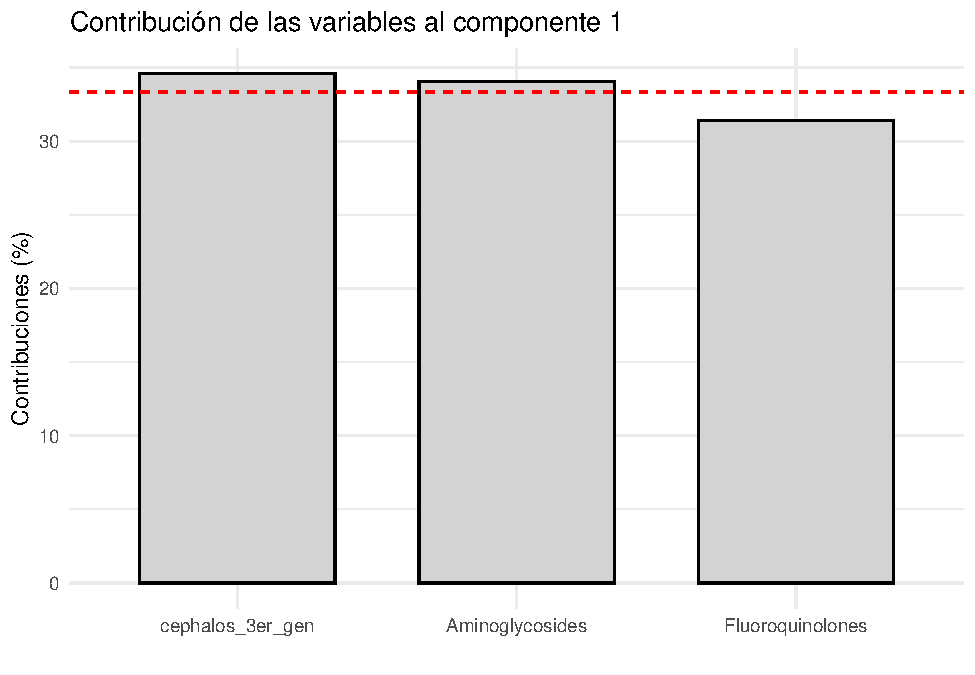
\includegraphics{2_actividad_PCA_files/figure-latex/GRÁFICA contribución 1-1.pdf}
\caption{Contribuciones de las variables en cada la componente principa
1}
\end{figure}

Seguidamente, se realiza una gráfica de contribuciones de variables a
las compomentes principales obtenidas. Esta información se encuentra en
la tabla 4. La gráfica de contribuciones, figura 2. Como se puede
observar, se realiza una discriminación por color dónde el color rojo
indica la máxima contribución de la variable al componente relacionado y
el colo azul es la menor. Si bien el vector de la variable
\texttt{Fluoroquinolones} se ve de color rojo por su alta contribución
no se hace al componente prinicipal 1, sino al 2. Aproximadamente el
68\% del compomente 2 es consecuencia de la variable
\texttt{Fluoroquinolones}. Mientras que su contribución en el compomente
1 es de 31.38\%.

\begin{figure}
\centering
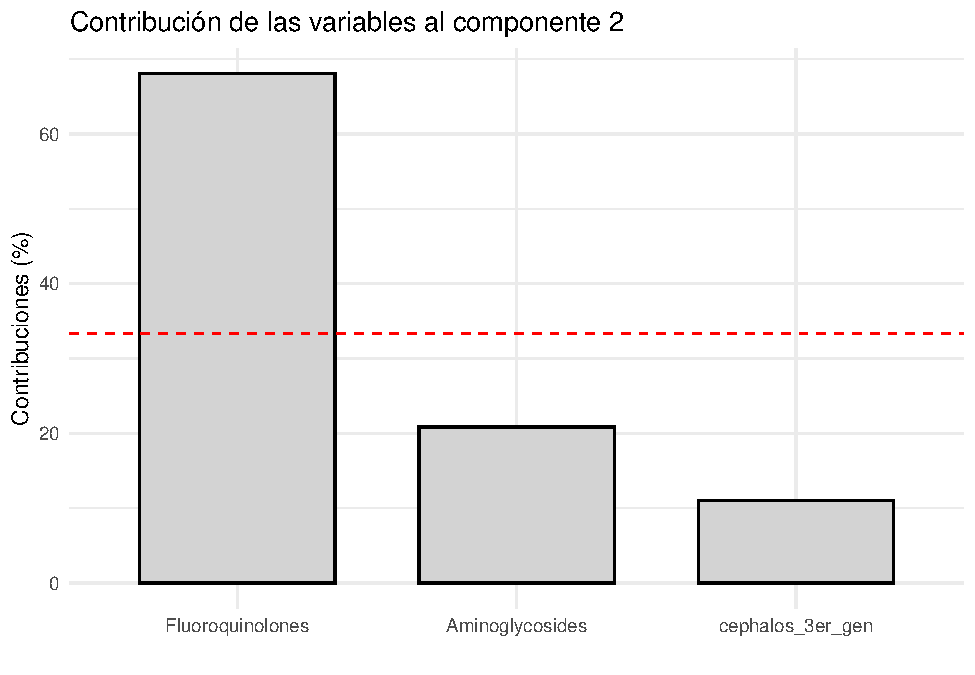
\includegraphics{2_actividad_PCA_files/figure-latex/GRÁFICA contribución 2-1.pdf}
\caption{Contribuciones de las variables en cada la componente principa
2}
\end{figure}

Cabe resaltar también el vector de la variable suplementaria
\texttt{Carbapenems} que como se predijo a través de los resultados
preliminares, contribuye muy poco en las componentes principales
resultantes. El peso de su contribución se da en color azul y la
distancia del vector desde el centro del plano es corta lo que sugiere
que contribuye poco a todas las compomentes, y su mayor contribución es
al componente 1.

Las figuras 4, 5 y 6. corresponde a gráficas de barras que comparan el
\% de contribucion de cada una de las variables para cada una de las
componentes principales. En cada una de estas gráficas se trazó una
línea roja que corresponde al contribución promedio esperada. Esto
indica que la variable que supere este valor umbrar contribuye más que
de lo esperado por las variables originales.

\begin{figure}
\centering
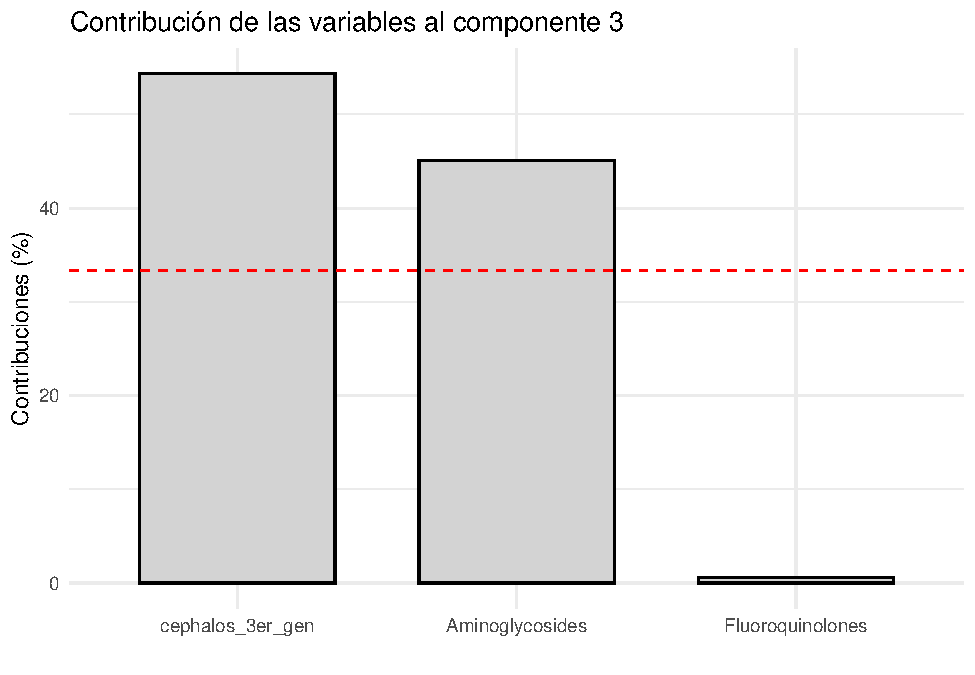
\includegraphics{2_actividad_PCA_files/figure-latex/GRÁFICA contribución 3-1.pdf}
\caption{Contribuciones de las variables en cada la componente principa
3}
\end{figure}

Por su parte, la figura 4. muestra que las variables
\texttt{cephalos\_3er\_gen} y \texttt{Aminoglycosides} son las que
contribuyen en mayor medida a la componente principa 1 en una medida
mayor que el la contribución esperada.

\begin{figure}
\centering
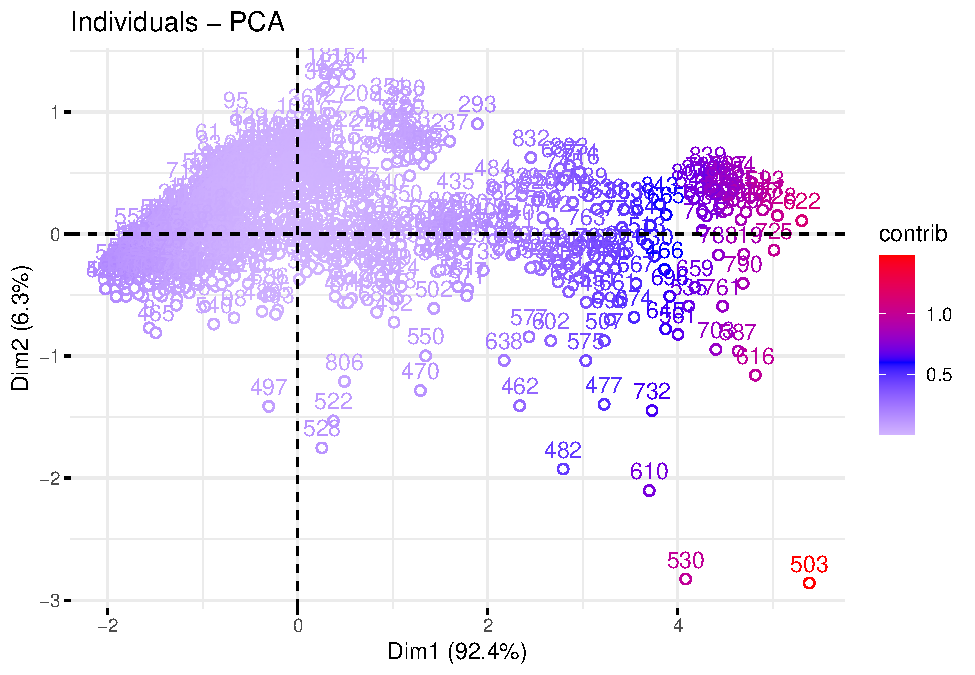
\includegraphics{2_actividad_PCA_files/figure-latex/GRÁFICA individuos por contribución 2-1.pdf}
\caption{Gráfica de la distribución y contribuciones de las
observaciones en las componentes principales}
\end{figure}

La figura 5. muestra que las variables \texttt{Fluoroquinolones} es la
que contribuye en mayor medida a la componente principa 2 en una medida
mayor que el la contribución esperada.

Finalmente la figura 6. muestra que las variables
\texttt{cephalos\_3er\_gen} y \texttt{Aminoglycosides} son las que
contribuyen en mayor medida a la componente principa 3 en una medida
mayor que el la contribución esperada; sin embargo, esta componente no
se puede obervar en las figuras 2 y 3, y tampoco es mandatorio retenerla
en este análisis.

Se Adicionó una gráfica de contribución de las observaciones en las
componentes principales (figura 7) en esta podemos obervar que la mayor
parte de las observaciones se encuentra cercanas al centro del plano
factorial. Sin embargo la dispersión de las observaciones tiende hacia
la derecha, es decir hacia el plano positivo del eje y, lo que
corresponde a la componente principal 1. Se realizó una discriminación
por color de la contribución: las observaciones de color rojo son las de
mayor contribución en las componentes y las de color más grisaceo son
las de menos contribución con una contribución intermedia las de color
azul. Como se puede ver las observaciones 530 y 503 (outsiders) son las
que más aportan en la componente 1 de manera individual.

\hypertarget{anuxe1lisis-multivariado-de-apc}{%
\subsubsection{Análisis multivariado de
APC}\label{anuxe1lisis-multivariado-de-apc}}

\begin{figure}
\centering
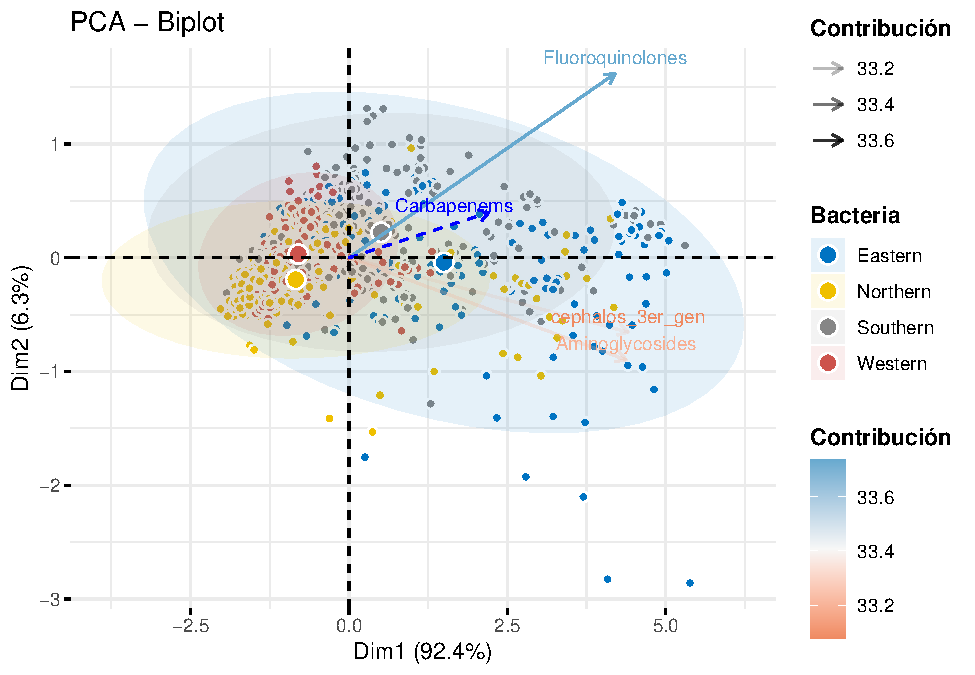
\includegraphics{2_actividad_PCA_files/figure-latex/GRÁFICA Biplot por región-1.pdf}
\caption{Gráfica de las componentes principales y la distribución de
observaciones por region}
\end{figure}

Se realizaron dos análisis más que pueden encontrarse en las figuras 8 y
9. Estos corresponde a un gráfico tipo \emph{Biplot} que permite hacer
discriminaciones de las observaciones en le plano factoria introduciendo
variables categóricas. Este análisis es particularmente interesante ya
que se realizó una discriminación de las observaciones en el plano a
través de especie de \texttt{Bacteria} (figura 9) y por \texttt{Region}
(figura 8).

La figura 8, preve algunos resultados que se verán en el análisis de
Clusters que se realizará más adelante. En este se encuentra que los
paises del este europeo \texttt{Eastern}son los que más contribuyen en
la componente principal 1. Aquí tambien se encuentran algunos países de
la región sur de europa y el norte, sugieriendo que los países del oeste
\texttt{Western} son los que menos contribuyen a la resistencia
antibiótica. En especial los paises del este contribuye a la resistencia
atibiótica de grupos como la Aminoglucosidos y las cefalosporinas de
tercera generación, que son antibióticos última línea para el
tratamiento de las infecciones producidas por estas dos bacterias.

\begin{figure}
\centering
\includegraphics{2_actividad_PCA_files/figure-latex/GRÁFICA Biplot por bacteria-1.pdf}
\caption{Gráfica de las componentes principales y la distribución de
observaciones por especie de bacteria}
\end{figure}

Por último, la figura 9, muestra un la dispersión de las observaciones
en le plano factoria y agrupadas por tipo de bacteria. Como se veía en
el primer análisis realizado, la bacteria Klebsiella Pneumoniae es la
que más contribuye a la resistencia antibiótica. Esto queda soportado,
dado que se evidencia una amplia diferencia en la distribución de las
observaciones que corresponden a esta en la componente principal 1,
particularmente interesante es que contribuyen a la a resistencia
atibiótica de grupos como la Aminoglucosidos y las cefalosporinas de
tercera generación y que aunado con los resultados de la figura 8, se
puede sugerir que el impacto mayor de esta resistencia es el los países
del este de europa.

\end{document}
